% !TEX TS-program = pdflatexmk
\documentclass[
12pt, % Main document font size
letterpaper, % Paper type, use 'letterpaper' for US Letter paper
oneside, % One page layout (no page indentation)
%twoside, % Two page layout (page indentation for binding and different headers)
headinclude,footinclude, % Extra spacing for the header and footer
BCOR5mm, % Binding correction
]{scrartcl}

\input{structure.tex} % Include the structure.tex file which specified the document structure and layout
\usepackage[top=0.75in, bottom=0.75in, left=0.75in, right=0.75in]{geometry}
\usepackage{hyperref}
\usepackage{aastex}
\newcommand{\blue}[1]{\textcolor{blue}{#1}}
\newcommand{\pb}{\textsc{Polarbear}}
\newcommand{\clbb}{$C_\ell^{BB}$}

\hyphenation{Fortran hy-phen-ation} % Specify custom hyphenation points in words with dashes where you would like hyphenation to occur, or alternatively, don't put any dashes in a word to stop hyphenation altogether

%----------------------------------------------------------------------------------------
%	TITLE AND AUTHOR(S)
%----------------------------------------------------------------------------------------

\title{\normalfont\spacedallcaps{Systematics Dictionary}} 
\author{} 
\date{} % An optional date to appear under the author(s)

%----------------------------------------------------------------------------------------

\begin{document}

%----------------------------------------------------------------------------------------
%	HEADERS
%----------------------------------------------------------------------------------------

\renewcommand{\sectionmark}[1]{\markright{\spacedlowsmallcaps{#1}}} % The header for all pages (oneside) or for even pages (twoside)
%\renewcommand{\subsectionmark}[1]{\markright{\thesubsection~#1}} % Uncomment when using the twoside option - this modifies the header on odd pages
\lehead{\mbox{\llap{\small\thepage\kern1em\color{halfgray} \vline}\color{halfgray}\hspace{0.5em}\rightmark\hfil}} % The header style

\pagestyle{scrheadings} % Enable the headers specified in this block

%----------------------------------------------------------------------------------------
%	TABLE OF CONTENTS & LISTS OF FIGURES AND TABLES
%----------------------------------------------------------------------------------------

\maketitle % Print the title/author/date block

\setcounter{tocdepth}{2} % Set the depth of the table of contents to show sections and subsections only

\tableofcontents % Print the table of contents

%\listoffigures % Print the list of figures

%\listoftables % Print the list of tables

%----------------------------------------------------------------------------------------
%	ABSTRACT
%----------------------------------------------------------------------------------------

\section*{Abstract} % This section will not appear in the table of contents due to the star (\section*)
A summary of systematics.

%----------------------------------------------------------------------------------------
\newpage % Start the article content on the second page, remove this if you have a longer abstract that goes onto the second page

%----------------------------------------------------------------------------------------
%	Input systematic files (Put your input here)
%----------------------------------------------------------------------------------------

\section{Introduction}
\input{tex/intro.tex}

\section{Optics}
\subsection{Systematic/Property Name}

\paragraph{Description:}
Description of systematic effect, including relevant equations and
parameterization for TWGs. Note that each variable in each equation should be
defined. This should include where we expect to get the value of this variable
from (TWG, literature, etc.)

\paragraph{Plan to model and/or measure:}
Plan to model/measure effect. Use TRLs to describe how well we understand/can model the effect. Is there a good null test that we could use to catch this effect?

\paragraph{Uncertainty/Range:}
This section should include the uncertainty of
known parameters and/or the expected range of parameters for consideration

\paragraph{Parameterization:}
This section should include the parameterization of figures of
merit and the output to the SWGs.

\subsection{Pointing}

\paragraph{Description:}
Pointing reconstruction is necessary in order accurate know where the instrument is looking at on the sky at any particular time. It is well known that many mechanical, structural, and environmental factors will affect the telescope pointing on the sky and a pointing model is needed in order to recover the pointing accuracy to the level needed for high ell science. The pointing systematics can be categorized into random pointing jitter, systematic pointing error, and optical pointing distortions.

Pointing models are very commonly used for astronomical telescopes in order to reconstruct accurate telescope pointing. Commonly used pointing model parameters are described in Mangum, 2001. Typically structural deformations and tilts, encoder offsets, and timing errors are taken into account through the pointing model. Pointing models are calculated through dedicated pointing observations of point-like sources across the sky in azimuth and elevation. Ideally uniform sampling across the sky is necessary but in many cases bright point-like sources are not available in various parts of the sky which can lead to errors in the pointing reconstruction.

Random pointing jitter is the statistical RMS error in the pointing reconstruction. In the case that the pointing error is random, this error can be modeling as a blurring or broadening of the telescope beam. Hence the effect is equivalent to decreased sky resolution. This can be modeled in terms of $B_{\ell}$
\begin{equation}
B_{\ell}^{eff} = B_{\ell} e^{\frac{-\ell(\ell+1)}{2} \sigma^{2}_{p,RMS}}
\end{equation}
where $\sigma^{2}_{p,RMS}$ is the RMS pointing error. 

The pointing error jitter can also have a similar effect as lensing: it mixes E-modes into B-mode \cite{hu03}:
\begin{align} 
\label{eq: bmodes from attitude errors pa}
p_A: \,\,\,\, \delta C_{\ell}^{BB} &= \int \frac{\mathrm{d^2} \vec{{\ell}}_1}{(2\pi)^2}   C^{EE}_{{\ell}_2}(\sigma) C^{\theta \theta}_{{\ell}_1} [\vec{{\ell}}_2 \cdot              \hat{{\ell}}_1 \sin[2(\Phi_{{\ell}_2} - \Phi_{\ell})]]^2 \\
\label{eq: bmodes from attitude errors pb}
p_B: \,\,\,\, \delta C_{\ell}^{BB} &= \int \frac{\mathrm{d^2} \vec{{\ell}}_1}{(2\pi)^2}   C^{EE}_{{\ell}_2}(\sigma) C^{\theta \theta}_{{\ell}_1} [(\vec{{\ell}}_2 \times            \hat{{\ell}}_1) \cdot \hat{z} \sin[2(\Phi_{{\ell}_2} - \Phi_{\ell})]]^2 
\end{align}
\noindent where  $\vec{{\ell}_2} = \vec{{\ell}} - \vec{{\ell}_1}$, $\sigma$ is the experiment Gaussian beam width, $C_{\ell}^{\theta \theta}$ is the power spectrum of the      attitude error in the map, and $p_A$ and $p_B$ stand for pointing effects A and B and should be added up in quadrature.
Note that in these equations, $C_{\ell}^{EE}(\sigma)$ is smoothed over the beam:  $C^{EE}_{\ell}(\sigma) = C^{EE}_{\ell} \exp{(-{\ell}({\ell}+1)\sigma^2)}$.
For a white noise pointing error with RMS $\sigma_{\theta map}$ and coherence scale $\ell_s$:

\begin{equation}
 C^{\theta \theta}_{\ell} \simeq \frac{2\pi\sigma_{\theta map}^2}{{\ell}_s^2}\exp(-\frac{{\ell}({\ell}+1)}{2{\ell}_s^2})
\end{equation}

\noindent the above spurious B-modes simplifies to

\begin{equation}
\delta  C_{\ell}^{BB} \simeq  \frac{1}{2}\frac{\sigma_{\theta map}^2}{{\ell}_s^2}         \int^{{\ell}_s} \mathrm{d}{\ell}_1 \ {\ell}_1^3 \ C^{EE}_{{\ell}_2}(\sigma)
\end{equation}


Systematic pointing error is the residual error in the pointing reconstruction dependent on external parameters. This pointing error is due to optical elements moving relative to each other causing optical misalignment. For example it is well known that thermal and solar heating and cooling of the telescope can cause large amounts of pointing error on the orders of 10s of arcseconds. An overall ambient temperature change can cause pointing drifts across time. Furthermore differential solar heating creating temperature gradients across the telescope structure can cause complex pointing changes that depend on the structural shape of the telescope itself. This error is difficult to model due to its complex dependence on telescope orientation and environmental parameters
\begin{equation}
\sigma_{p,sys} \left ( Az, El, T, I_{R}, v_{w}, ... \right )
\end{equation}
In the case that there is uniform sampling across each of these parameters and the errors are small relative to the beam size, then the pointing error can be roughly approximated similar to the pointing jitter, but this may not always be the case. If the systematic nature is complex, then the effective beam may become non-Gaussian in ways difficult to model.

Optical pointing distortions are pointing errors due to deformation of the optical elements themselves. This error is distinguished from systematic pointing errors above in that the optics itself changes rather than just alignment. For example the primary mirror can deform due to solar heating during the daytime and change the F number of the system. Pointing distortions are harder to correct than systematic pointing error because they are dependent on the tolerance of the optical system and hence affect the optical performance of the telescope. Typically the effects are larger in degree than the other pointing errors and may only be correctable by active realignment of the telescope itself or insulating optical elements well.
\begin{equation}
\delta_{p} \left ( x, y, M, ... \right )
\end{equation}
Here $M$ represents the Mueller matrix beam model calculable through physical optics simulations. 

\paragraph{Plan to model and/or measure:}
Frequent and regular observations of bright point-like sources across the sky are needed in order to calculate a pointing model. With good coverage across azimuth and elevation, the pointing jitter can be minimized well. With good coverage the jitter error will eventually be limited by errors in the analysis itself such as fitting for beam centroids.

This pointing model can be expanded to include parameters that model environmental effects as done in POLARBEAR. This would allow for modeling and minimizing the systematic error, but there is a limit to how well these effects can be corrected using the pointing model alone. Regular observations around the year as well as at various times during the day will be needed to assess the impact of this error and its dependence to the environmental parameters.

Optical pointing distortions need to be mainly modeled using physical optics or structural analysis of the optical elements under various environmental conditions. This is by far the hardest to model and measure.

Several formalism exist to model the effect of pointing errors onto the measured B-modes \cite{hu03, Shimon_2008}, involving convolving the power spectrum of the pointing error with sky signal to measure the spurious signals generated. For SO this \href{http://simonsobservatory.wdfiles.com/local--files/calandsys-telecon/eb_leakage_from_pointing_error.pdf?ukey=61f26ef33e8439a4e7096ab52c54c523066a4e35}{memo} investigates briefly how pointing errors lense E-modes into B-modes. Linking the pointing error at the level of the map to telescope models and instantaneous pointing errors needs more work.

\paragraph{Uncertainty/Range:}
Telescope pointing specs requirements are of order 10 arcseconds.
\cite{didier_memo17} shows that white noise pointing errors with RMS=9 arcseconds and coherence length 1000 creates spurious B-modes of order 10\% of sky B-modes starting $\ell \sim 1,000$.

\paragraph{Parameterization:}
For linking pointing errors to science: use the power spectra of the pointing error at the level of the map, $C_l^{\theta \theta}$.
To obtain this, need to model the time- or az/el-dependant pointing error and link this with a scanning strategy.

\subsection{Beam ellipticity}

\paragraph{Description:}
Many CMB experiments are designed to have angular sensitivity that can be described by an azimuthally symmetric two-dimensional Gaussian function
\begin{equation} 
P (\mathbf{x}) \propto \exp (-\mathbf{x} ^2/2\sigma ^2),
\end{equation}
where $\sigma$ represents the width of the beam. Optical aberrations will lead to asymmetries in the angular sensitivity which can often be captured by assuming that the Gaussian beam width is different along the two axis of a Cartesian coordinate system centered on the peak response
\begin{equation}
P (x,y) = \frac{1}{2\pi \sigma_x \sigma_y} \exp (-\frac{1}{2}[x^2/\sigma ^2_x + y^2/\sigma ^2_y]).
\end{equation}
This is referred to as an elliptical Gaussian function. The $\sigma_x$ and $\sigma_y$ parameters are the widths of the elliptical Gaussian beam along its two principal axes. The beam full width at half maximum (FWHM) can be defined 
\begin{equation}
\theta _\mathrm{FWHM} = \sqrt{8\sigma_x \sigma_y\log{(2)}}. 
\end{equation}
We define beam ellipticity as 
\begin{equation}
e = (\sigma_x-\sigma_y)/(\sigma_x+\sigma_y)
\end{equation}
\textbf{Is this the standard definition for beam ellipticity? I have seen the same but squared quantities: $e = (\sigma_x^2-\sigma_y^2)/(\sigma_x^2+\sigma_y^2)$}. The beam ellipticity quantifies the extent to which the symmetry of the detector spatial response is broken. A highly elliptical beam response suggests that the detector signal response at any given time is dependent on the orientation of your detector relative to the signal on the sky; in other words, your scan strategy.

The spherical harmonic transform of an elliptical Gaussian beam is discussed in \cite{Souradeep2001}. Let's try \cite{Takahashi2010}.

\paragraph{Plan to model and/or measure:}
Beam widths and ellipticities are extracted from beam maps which are acquired through scanning of a terrestrial source placed in the far-field of the optical system or by observing astrophysical point-sources such as the planets in our solar system. 

An attempt to model it and propagate it through the systematic pipeline can be found at \href{http://simonsobservatory.wikidot.com/instrument-systematic-systmodule#toc5}{here}. This study focuses on the v2 configuration for the instrument. \textbf{Question: should I expand here the analysis and remove the link to the wiki? Or just a link to the wiki is ok?}

\paragraph{Uncertainty/Range:}
Insert text

\paragraph{Parameterization:}

% !TEX root =  ../syst_master.tex 

\subsection{Cross Polarization}

\paragraph{Description:}
Cross polarization is an optical systematic that shows how much polarization leakage there is between orthogonal polarization modes. Typically it is a characteristic of the optical design itself and represents how much polarization is rotated as it propagates through the optics. Alternatively, it can comes from differencing detectors with different beam shapes.

This can be calibrated out with accurate polarization angle calibration but does decrease polarization efficiency. If the calibration is incorrect, this will cause Q and U to leak into each other and cause E modes leaking into B modes. 

It can be modeled using the Mueller matrix formalism. If the telescope Mueller beam matrix is known, these systematics (along with beam effects) can be propagated to the Q, U maps by
\begin{equation}
Q' = m_{qq} Q + m_{qu} U, \ \ U' = m_{uu} U + m_{uq} Q
\end{equation}
In this way systematics contaminated Q and U maps can be simulated. The contaminated Q and U maps can be further propagated to the power spectra to see the leakage effect.

\paragraph{Plan to model and/or measure:}
This effect can be modeled using physical optics simulations where the Mueller matrix can be calculated directly. Comparing this to real data may be needed using a polarized source.

\paragraph{Uncertainty/Range:}
Insert text

\paragraph{Parameterization:}
Insert text

\subsection{Instrumental Polarization} 
\label{instrumental_polarization}

Instrumental polarization (IP) is an optical systematic that shows how much intensity signal is leaking into the polarization signal. It can come from the optics (depends on the properties of metals and dielectric materials), or come from pair differencing with detectors having different beams. For optical elements, different transmission along orthogonal axis will polarize incoming unpolarized light. The optical components also emit polarized light for the same reason, but with opposite polarization angle.
This systematic will leak the T signal into E and B modes causing large contamination if not accounted for in analysis.

It can be modeled using the Mueller matrix formalism. The effect is worse at the edge of the focal plane because of the increased incident angles on optical elements. If the telescope Mueller beam matrix is known, these systematics (along with beam effects) can be propagated to the Q, U maps by
\begin{equation}
Q' = m_{qq} Q + m_{qi} I, \ \ U' = m_{uu} U + m_{ui} I
\end{equation}
In this way systematics contaminated Q and U maps can be simulated. The contaminated Q and U maps can be further propagated to the power spectra to see the leakage effect.

\paragraph{Plan to model and/or measure:}
\noindent Intrinsic Optical Leakage: \\
This effect can be modeled using physical optics simulations where the Mueller matrix can be calculated directly. 
The main optical elements to consider are mirrors, lenses, and filters.
A study of IP of filters can be found in \cite{pisano2005}.

The combined IP of the windows and lenses for ACTPol was calculated using Code V, 
by putting an unpolarized input on the sky and propagating it to the focal plane.
The IP is larger towards the edges of the detector due to the non-zero incident angles.
This gives values of $\sim0.12\%$ and $\sim0.015\%$ at the edges and the center respectively.
For now we assume that this IP is divided equally among the lenses.

Optical leakage also occurs at the mirrors due to their finite conductivity. 
The formula is calculated in \cite{Barkats:2005sh}, and is given by the Hagen-Rubens formula multiplied by 
a geometric factor determined by the incident angle:
\begin{equation}
\lambda_\text{opt}(\nu) = \sqrt{4 \pi \epsilon_0 \nu \rho} (\sec \chi - \cos \chi).
\end{equation}
where $\rho$ is the conductivity of the mirror and $\chi$ the incident angle.

Currently we use the mirror specifications of CCAT, which gives incident angles of $25.73^\circ$ for the primary mirror 
and $19.59^\circ$ for the secondary. The IP of both mirrors together ends up around $0.04\%$ at 145 degrees.

In the case of a HWP, only the IP up to the HWP needs to be considered.
A more detailed discussion of how to calculate the power coming from IP and instrumental polarization
seen by the detector is given in section \ref{HWP Differential Optical Properties}.
A first attempt at tallying up the IP from the optical chain in SO is available in this \href{http://simonsobservatory.wdfiles.com/local--files/calandsys-telecon/eb_leakage_from_pointing_error.pdf?ukey=61f26ef33e8439a4e7096ab52c54c523066a4e35}{memo}.


\noindent Pair Differencing Leakage: \\
The framework to simulate this is in the systematics pipeline as described in details in \url{http://simonsobservatory.wikidot.com/instrument-systematic-systmodule#toc5}.
See Beam Ellipticity section for more details.

\paragraph{Uncertainty/Range:}
Using the methods above for the lenses and mirrors, we see an IP of about $0.16\%$ for the whole system.
A more detail study integrates all incident angles over each optical elements, and add up the IP of various elements  coherently.

\paragraph{Parameterization:}
Instrument mueller matrix elements $m_{qi}$ and $m_{ui}$ as a function of frequency and incident angle.



\subsection{Polarization Angle}

\paragraph{Description:}
% Description of systematic effect, including relevant equations and
% parameterization for TWGs. Note that each variable in each equation should be
% defined. This should include where we expect to get the value of this variable
% from (TWG, literature, etc.)

Sources of polarization angle systematics are varied and can be introduced
several places in the instrument. To name a few examples, 1) a rotating elliptical beam (say
in the case of a design incorporating bore-sight rotations) can cause T to P
leakage, 2) off axis refractive optics influence the propagation of the
polarization vectors according to their Fresnel coefficients leading to an
instrumental polarization angle rotation and 3) in the presence of a HWP an
apparent polarization angle rotation can arise from the detector time
constants. 

Perhaps 1) and 3) are best left to their respective sections on beams and time
constants. Here we focus on 2), namely instrumental polarization errors and
detector polarization angle rotations. Understanding this instrumental
polarization error has implications not only for measuring CMB polarization,
but for placing constraints on Cosmic Polarization Rotation (CPR).

A global polarization rotation is degenerate with a CPR angle and affects the
power spectra as described in \cite{2013ApJ...762L..23K}. Analytic description
of instrumental rotation is challenging, necessitating the use of optical
modeling and experimental techniques for calibration of final detector angles
(absolute and relative) and systematic rotations from the optics.

\paragraph{Plan to model and/or measure:}
%Plan to model/measure effect
We should plan to both model and measure the detector polarization angles.
Calibration should be performed before deployment and during observations. This
can be done with a lab calibrator as well as an astrophysical polarized
source. Polarized sources already used as references include Tau A (the Crab
Nebula) and Cen A.

When considering a lab source, placing a well known polarization
calibrator in the far field is preferred, though difficult in practice.
Proposed ideas include flying a source (whether tunable or wide band) on a
drone or on a CalSat to place it in the far field. Alternative calibrators
require placement in the near field and include sparse/dense wire grid
polarizers or dielectric sheets \cite{Takahashi2010, 2016arXiv160701825K}.

Modeling of the polarization rotation angle appears feasible and has been used
on ACTPol using Code V \cite{2016arXiv160701825K}. This should be checked with
physical optics calculations, but can be performed on a proposed telescope
design.

\paragraph{Uncertainty/Range:}
%This section should include the uncertainty of
%known parameters and/or the expected range of parameters for consideration

Angle offsets $\sim 1^{\circ}$ produce spurious B-mode signal at the same level
as primodial B-modes for a tensor to scalar ratio $r \sim 0.005$ as well as
nonzero $EB$ and $TB$ cross-correlations \cite{doi:10.1142/S0218271816400125}.
Currently employed calibration methods provide calibration to at best
$0.5^{\circ}$ \cite{2016MNRAS.455.1981K}. Calibration to better than
$0.05^{\circ}$ would allow for constraints on CPR of order one degree to
greater than $15\sigma$ \cite{2016MNRAS.455.1981K}.

\paragraph{Parameterization:}
%This section should include the parameterization of figures of
%merit and the output to the SWGs.



\section{Spectral Response Function}
\input{tex/bandpass_mismatch.tex}

\section{Polarization Modulators}
An ideal HWP is made of a birefringent material and flips the polarization of incoming light along the fast axis of the crystal resulting in a polarization shift of $2\chi$, where $\chi$ is the incoming polarization angle of the light with respect to the fast axis. Thus, a HWP rotating with frequency $f_{m}$ modulates the incoming polarization at $2f_{m}$, which is detected in the bolometer timestreams at $4f_{m}$. The demodulation process described below summarizes the formalism defined in Kusaka \& Essinger-Hileman et al., 2014~\cite{ABS_HWP} and is an excerpt from~\cite{Simon_Thesis_2016}.

The detector timestream $d_{m}$ is composed of the unpolarized sky intensity $I$, the modulated polarization signal $P(\chi)$, white noise $N_{w}$, and spurious modulation signals $A(\chi)$ that depend on the HWP angle $\chi$ such that
\begin{equation}
d_{m}= I + P(\chi)+ N_{w} + A(\chi).
\end{equation}
The modulated polarization signal can be represented in terms of the Stokes $Q$ and $U$ parameters (Equation~\ref{eqn:Stokes_QU}) as
\begin{equation}
P(\chi)=\epsilon \mathrm{Re}\{(Q+iU) m(\chi)\},
\end{equation}
where the modulation is given by $m(\chi)=\exp[-4 i \chi]$ and $\epsilon$ is the polarization modulation efficiency factor, which is close to one. The spurious modulation signals $A(\chi)$ consist of components at every harmonic $n$ of the HWP rotation frequency and can be decomposed into cosine and sine components as
\begin{equation}\label{eqn:achi}
A(\chi)= \sum_{n} A_n(\chi)=\sum_{n}\Big[ (A^{nc}_{0} + \lambda^{nc} I) \cos(n\chi) + (A^{ns}_{0} + \lambda^{ns} I) \sin(n\chi)    \Big].
\end{equation}
Here the $A_{0}$ terms are stable and independent of the sky intensity and the $\lambda$ terms are small~\cite{ABS_HWP}.

The demodulated timestream is then determined by applying a bandpass filter to $d_{m}$ to account for the slight variations in $f_{m}$, multiplying $d_{m}$ by $m^*(\chi)$, and applying a low-pass filter that passes $f\lesssim2$~Hz to eliminate higher order terms and all $A^{nc,s}$ and $\lambda^{nc,s}$ terms other than the $n=4$ components. From~\cite{ABS_HWP}, the final demodulated timestream $d_{\bar{d}}$ is then given by
\begin{equation}
d_{\bar{d}}=\frac{1}{2}\Big(\epsilon Q + A^{4c}_{0} + \lambda^{4c} I \Big) + N^{\mathrm{Re}}_{w} + \frac{i}{2}\Big(\epsilon U + A^{4s}_{0} + \lambda^{4s} I \Big) + iN^{\mathrm{Im}}_{w}.
\end{equation}

\subsection{Differential Optical Properties of a HWP}

\paragraph{Description:}
Differential transmission, reflection and emissivity creates a $2$f component in a polarimeter exploiting a rotating HWP
\cite{Salatino10}. 

\paragraph{Plan to model and/or measure:}
Plan to model: HFSS model of the metamaterial HWP, transfer matrix method for the Sapphire HWP.
Plan to measure:
differential transmission and reflection: FTS measurements;
differential emissivity: HWP emissivity measurements at different temperatures
(liquid nitrogen, room temperature and temperatures higher than room temperature).

\paragraph{Uncertainty/Range:}
Transmission and reflection measured at room temperature scaled to cryogenic temperatures, same for differential emissivity.

\paragraph{Parameterization:}
12 Mueller matrix top left components of a real HWP or eq.$\,$(7) and (8) in \cite{Salatino16}. 

\subsection{Thermal Variation in HWP Temperature}

\paragraph{Description:}
HWP thermal gradient and thermal fluctuations. A not uniform HWP temperature and its temporal fluctuations create a spatial and time dependent 2$f$ signal.

\paragraph{Plan to model and/or measure:}
Model: thermal finite element analysis of a HWP thermalized with a suitable heat sink and with a realistic time variable loading.
Measure: cryogenic measurements of the thermal gradients.


\paragraph{Uncertainty/Range:}
Realistic model of the time variation of the loading.


\paragraph{Parameterization:}
HWP thermal fluctuations: $\Delta_{HWP}(x,y,t)$ with $(x,y)$ the spatial coordinates of the HWP and $t$ the time.


\subsection{HWP Beam Systematics}


\paragraph{Description:}
Putting a HWP skyward of every optical element cures a range of beam and polarization systematics. However, putting a HWP inside the optical system induces some beam and polarization systematics of its own, and fails to cure some systematics you'd think it would. Thus, careful consideration is needed.

\paragraph{Plan to model and/or measure:}
Modeling would entail ray tracing and physical optics for a non-planar or non-uniform AR coated HWP. It would also require calculating the impact of non-uniform AR coatings or optical properties. Non-normal incidence effects...might matter...might focus the beam...ask ABS people on the theory side, and PB/ACT people on the experience side.

Also model how these beam systematics show up in the rapid-rotation demodulation. Even with an optimal mapmaker, ignoring this effect would mean they will show up likely as I-P and Q-U leakage beams with very funny structure. (Investigate making an optimal mapmaker for this..? Would definitely require data since the dipole-quadrupole small-distortion beam formalism may not apply here.)

In general, CST is commercial software that can model diffraction, without too much CPU time, from very funny shaped large structures (like struts and baffles and things). Putting the HWP into that model to get some of these beam systematics might be interesting.

Measurements, in principle, would be done with a long campaign of beam maps taken at a large set of HWP angle. And/or, in the case of a rapid modulator, very slow beam maps taken with several modulation cycles per beam scanned (unlike in science mode where we can scan fast). The source is TBD, a sky source seems like it would be slow, and informally in the meeting people were saying that a source on a mast will be difficult because it requires tilting the telescope to a low elevation that's mechanically difficult.

\paragraph{Uncertainty/Range:}
Very uncertain "prior" on this, could be no effect, could be huge and a showstopper.

\paragraph{Parameterization:}

Leverage existing beam formalisms? Leverage Maria, Sean, Tom E-H, others, work on polarization non-idealities of the HWP, but combine it with beam formalisms?

\subsection{Encoder Jitter}

\paragraph{Description:} 
% Description of systematic effect, including relevant equations and
% parameterization for TWGs. Note that each variable in each equation should be
% defined. This should include where we expect to get the value of this variable
% from (TWG, literature, etc.)

A source of white noise in the demodulated timestream is encoder jitter, which is governed by how well the HWP angle and bolometer sample are matched in the time-ordered data (TOD). 

During observation, the HWP angle and bolometer samples are read out and timestamped simultaneously by a global trigger, sent to a centralized DAQ device, and paired within a single data packet. In an ideal world, the HWP angle assigned to this timestamp will be correctly obtained and synchronized; however, in reality, the stored HWP angle is not exact but instead exhibits some (presumedly Gaussian white) distribution around the true value. This ``angle jitter'' creates a decorrelation between the rotation-synchronous signal of the HWP and the signal detected by the bolometers. During analysis, this error between the HWP angle the the ``true'' angle experienced by the bolometer (via the HWP-synchronous signal) injects white noise into the demodulated timestream.

Below are a few sources of this timestamp jitter:

\begin{itemize}
 \item \textbf{A noisy encoder waveform} creates a jitter in the interpereted angle of the HWP for each encoder tick. Casues of waveform-induced noise include poor sensor signal-to-noise, a waveform with poorly-defined rising and falling edges (e.g. sloping rather than sharp edges), noisy waveform amplification, and non-rotation-sychronous HWP rotor vibrations.
 \item \textbf{An inadequate encoder sampling rate} prevents precise identification of the encoder ticks. If your encoder readout is sampling the encoder slowly, inerpolation must be used to estimate the HWP angle. Interpolation relies on the smoothness of the HWP rotation and therefore can be noisy if the HWP is vibrating or wobbling.
 \item \textbf{An inadeqaute encoder tick frequency}, in a similar way to an inadequate sampling rate, requires a reliance on interpolation to retrive the HWP angle and therefore can be noisy.
 \end{itemize}
  
\paragraph{Plan to model and/or measure:}
%Plan to model/measure effect

Expected instrumental polarization from optical elements in front of your HWP must be modeled in order to make estimates of the expected power at 4f. This should be modeled using a physical optics simulator with realistic emissivities. Additionally, HWP differential emission and differential reflection should be measured prior to deployment to make estimates of the expedted power at 2f. Then, given these expected weights, you can set a requirement on the acceptable white noise for your amplifiers, on the well-behavedness of your encoder waveform, etc.

\paragraph{Uncertainty/Range:}
%This section should include the uncertainty of
%known parameters and/or the expected range of parameters for consideration

This systematic is driven by the size of the 2f and 4f signal of the HWP, which in turn is dependant on the instrumental polarization sky-side of the modulator. So, for a HWP at prime focus in the Cross-Dragone scenario, (POLARBEAR), the requirement is quite tight--less than 1 arcsecond--where as for a modulator at the stop of a small-aperture telescope (e.g. ABS), the requirement becomes looser.

This effect can be averaged down in analysis with interpolation schemes, and is hence improved if the HWP rotational stability is very good over long timescales.

\paragraph{Parameterization:}

The NET induced by this angle jitter is set by the size of the HWP-synchronous signal:
 
 \begin{equation}
 	NET_{jitter} = \frac{\mathrm{d}T}{\mathrm{d}\theta} \sigma_{\theta} 
 \end{equation}

As an example for how to set a requirment on angle jitter, let's say a HWP has a peak-to-peak 4f signal of 0.2 K and that you want to inject $< 10 \%$ white noise into your Q and U channels compared to your per-polarization array sensitivity of 5 $\mu K \sqrt{s}$. You then use the following relations to calculate $\sigma_{\theta}$

\begin{equation}
	\frac{\mathrm{d}T}{\mathrm{d}\theta}  = \frac{0.1 K}{\pi/8 rad}
\end{equation}

where we've assumed that the Q/U signal rises/falls by $A_{p2p}/2$ in $1/16$th of a HWP rotation (i.e. 4f). Then, the angle jitter requirement is given by

\begin{equation}
    	\sigma_{\theta} < \frac{\mathrm{d}\theta}{\mathrm{d}T} NET_{jitter} <  \frac{\pi/8 rad}{0.1 K} (0.5 \mu K \sqrt{s}) < 1.9 \mu rad \sqrt{s}
\end{equation}

The requirement gets tighter the larger your HWP sychrnous-signal is, hence making large instrumental polarization signals in front of your HWP dangerous.

To convert this angle requirement into a timestamp jitter, which is often more useful for diagnosing aspects of the system like IRIG and RP synchronization, microcontroller performance, etc., you divide the angle jitter by the HWP rotation speed. For the above example, for a 2 Hz HWP, the timestamp jitter requireent is

\begin{equation}
	\sigma_{t} = \sigma_{\theta} / \frac{\mathrm{d}\theta}{\mathrm{d}{t}} = (1.9 \mu rad \sqrt{s}) / (\frac{4 \pi}{s}) = 0.15 \mu s \sqrt{s}
\end{equation}

Again, the requirement on the HWP timestamp accuracy is made tighter as the HWP is spun faster.

\subsection{Sapphire HWP Degredation Over Time}

\paragraph{Description:} 
% Description of systematic effect, including relevant equations and
% parameterization for TWGs. Note that each variable in each equation should be
% defined. This should include where we expect to get the value of this variable
% from (TWG, literature, etc.)

One concern for the HWP is degredation of the modulator performance over time. A few causes for such degredation are

\begin{enumerate}
	\item AR coating delamination
	\item AR coating degredation, for instance due to UV-induced deterioration
	\item Birefringent substrate material degredation, for instance due to cracking
	\item Birefringent substrate moving around inside the rotor, therefore adjusting its angle with respect to the encoder
	\item HWP becoming dirtied by the environment
\end{enumerate}

POLARBEAR is now in its third season using a modulator \cite{PB1_WHWP}. The PB HWP consists of a sapphire sustrate with a layer of RT6002 Duroid from Rogers Corporation glued using melted LDPE for AR. The HWP is located between the primary and secondary mirrors (i.e. at prime focus) and is covered with a thin Mylar sheet for environmental protection. PB has not seen evidence of HWP degrdation despite snowstorms, windy weather, etc. The Mylar sheet should ideally be cleaned periodically.

For the POLARBEAR-2a warm HWP (WHWP) \cite{PB2a_WHWP}, we are using a three-stack sapphire HWP with RT3006 Duroid/HDPE dual-layer AR held onto the sapphire using a vacuum-bag technique (i.e. no glue layers). The HWP sits in front of the optics tube window and is protected from the environment by a weather-sealed boom enclosure. The vacuum technique avoids the possibilities of AR delamination and non-uniform glue-layers. To prevent the three sapphire plates from rotating with respect to one another, we epoxy them together at the edges, and to prevent the stack from shifting in the rotor, it is held snugly by a rubber gasket as well as the friction of the vacuum bag. Another concern for HWP degredation is UV eroding the HDPE quality, but we expect this effect to be small given the UV-tight quality of the boom enclosure.

For the POLARBEAR-2b/c cold HWP (CHWP), we are using three-stack sapphire with alumina thermal spray loaded with nitrogen-infused silica microspheres to adjust the dielectric constant. The HWP will sit behind the cryostat window at the 50 K stage. An additional concern for the CHWP is the danger of AR delamination due to differential thermal contraction during thermal cycles. However, the alumina-powder-based thermal-spray AR has the same expansion coefficient as the sapphire substrate, and no delamination has been seen in testing.
  
\paragraph{Plan to model and/or measure:}
%Plan to model/measure effect

For the WHWP, because it is outside the receiver, load curves can be taken by doing in-and-out tests between seasons to look for uniform degredations of the dielectric layers that would cause an increase in emission. 

Non-uniform degredations, such as AR delamination, will show up in the HWP-synchronous-signals, or if egregiuos enough, in beam maps. These effects, though, depend on where your HWP is located within the optical system.

\paragraph{Uncertainty/Range:}
%This section should include the uncertainty of
%known parameters and/or the expected range of parameters for consideration

The acceptable range of these effects are difficult to quantify, but we should not tolerate AR delamination or shifting of the birefringent substrate in the design process. If it happens in the field, we must hope it's dramatic enough that we see it immediately.

\paragraph{Parameterization:}

Parameters to pay attention to from the perspective of sensitivity:

\begin{enumerate}
	\item HWP efficiencyas a function of time $\eta(t)$
	\item HWP emissivity as a function of time $\epsilon(t)$
	\item HWP loading due to scattering as a function of time $P_{HWP, \, scatter}(t)$
\end{enumerate}	


\section{Time Constants}
The time constant of each detector is a key property that describes the stability and time response of the detector. If the time constant is too large, it must be accounted for in the demodulation of the signal from the HWP polarization modulation, in setting the scanning frequency of the telescope, in measuring the telescope beams and pointing, and in determining the polarization angles of the detectors (if using a HWP). The optical time constant $\tau_{opt}$ is often expressed in terms of the 3dB frequency $f_{3 dB}$, which is given by $f_{3dB}=1/(2\pi \tau_{opt})$. There are several ways to measure the detector time constants.

\paragraph{Planet Scan Method} The time constants of the detectors can be probed by scanning quickly over bright objects such as planets, but our ability to probe such features might be limited by the maximum scan speed of the telescope mount and the low signal to noise on an individual planet scan.

\paragraph{Bias Step Method} The bias step method characterizes the electrical time constant of a detector $\tau_{el}$ by inputing a low amplitude square wave through the bias line and fitting the exponential response. The current $I$ as a function of time $t$ goes as
\begin{equation}
I(t) \propto e^{\frac{\pm t}{\tau_{el}}},
\end{equation}
where the exponential is positive as the voltage is increased and negative as the voltage is decreased. The bias step method is quick and easy to perform before measurements, but $\tau_{el}$ must be properly correlated to optical time constant measurements to determine the optical time constant $\tau_{opt}$.

\paragraph{Amplitude Method} With the amplitude method, the time constants are determined by modulating a source with a chopper at various frequencies and measuring the amplitude of the detector responses with the HWP stationary (if using one). The response in power $P$ of the detectors is given by
\begin{equation}\label{eqn:tc_amp}
P(f) \propto \frac{1}{1+\Big(\frac{f}{f_{3dB}}\Big)^2},
\end{equation}
where $f_{3dB}$ is the optical 3dB frequency and $f$ is the modulation frequency of the source. Figure~\ref{fig:tc_chopper} shows the power versus frequency measurements from two measurements on ABS with their fits.

The optical time constant of a detector increases with increasing loading, and with this method, the added loading from the atmosphere near the horizon behind the source can be large enough to drastically slow the detector time constants and, in some cases, fully saturate the detectors, making them non-responsive. Thus, the time constants measured with this method may not be representative of the time constants under typical loading conditions. For example, in ABS, this method gave $f_{3dB} \sim 30$~Hz versus the actual average across the whole season of 109~Hz. Additionally, the measured amplitudes can be highly sensitive to changes in loading correlated to the weather. Without the use of the HWP, the atmosphere can cause fluctuations in the signals on order of a pW. The power versus frequency plot in the left panel of Figure~\ref{fig:tc_chopper} shows that the fluctuations can be larger than the effect from the time constants.

\begin{figure}[h!]
\centering
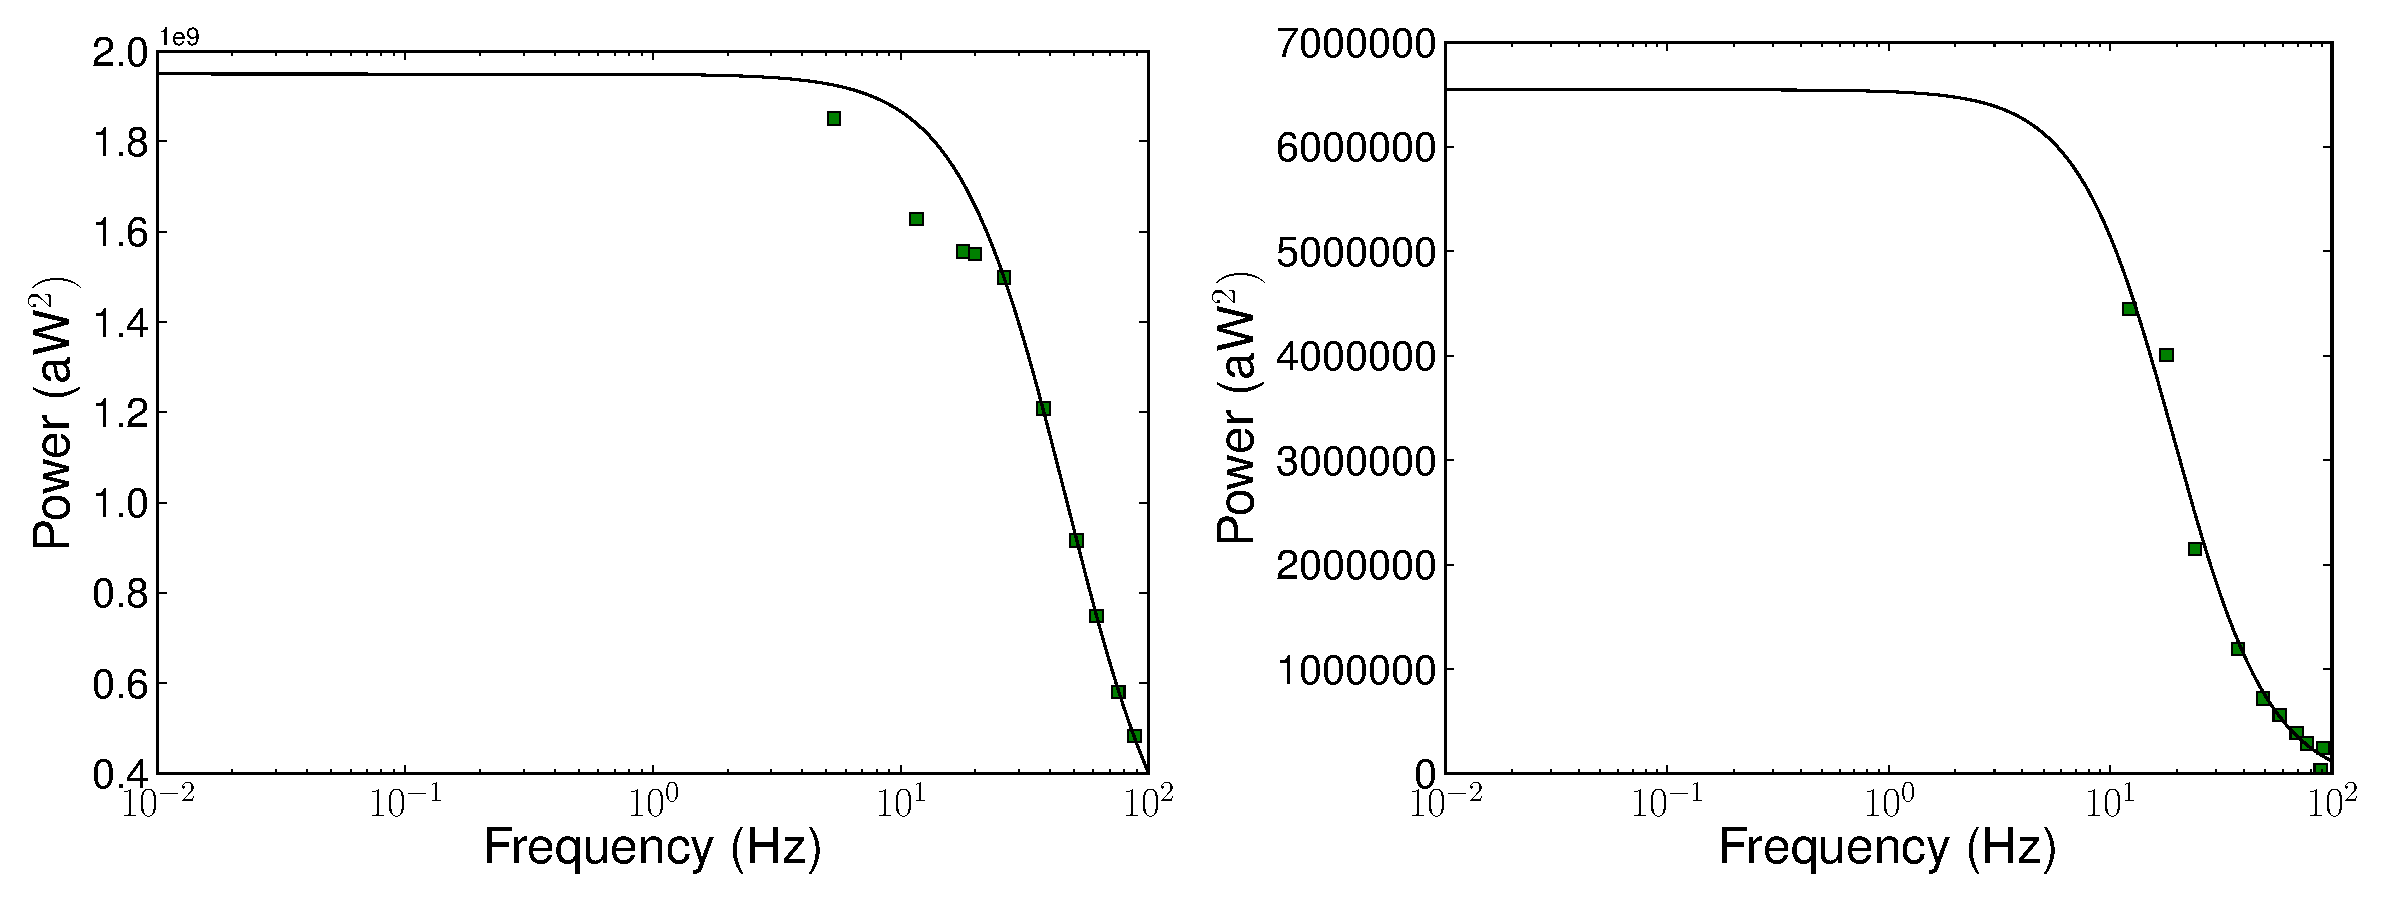
\includegraphics[width=\textwidth]{figures/ampl_pvfreq.pdf}
\caption{The power versus frequency relations are shown above in green with their fits in black for two time constant measurements on ABS. The large atmospheric fluctuations in the first four frequencies of the first measurement and in the last frequency of the second measurement cause the power to fluctuate more than the effect from the time constant, which can be problematic.}
\label{fig:tc_chopper}
\end{figure}

\paragraph{Phase Method} When an experiment has a HWP, the optical time constants can be characterized using the phase delay of the $4f_{m}$ signal~\cite{Simon_LTD2013}. Because it uses the phase, this technique is less susceptible to atmospheric fluctuations over the course of the measurement than the amplitude method. For each phase method measurement, data are taken while slowly varying the rotation speed of the HWP with a sparse polarizing wire grid made positioned above the HWP. The wire grid is used to input a small ($\sim0.1$ pW) polarized signal. This signal adds minimal loading, so the time constants are closer to those during nominal observation. The phase $\phi$ found from demodulating the signal with respect to the polarization modulation frequency $4f_{m}$ is the difference between the physical polarization angle of the grid and the measured polarization angle, which includes the apparent angle rotation due to the time delay of the detector response. It can be modeled as the phase of a one-pole filter: 
\begin{equation}\label{eqn:phi_shift}
\phi=\arctan{\left(\frac{4f_{m}}{f_{3dB}}\right)} + C,
\end{equation}
where $f_{3dB}$ is the optical 3dB frequency of the detector. Because $(4f_{m})^2$ is expected to be much less than $f_{3dB}^2$, the phase can be linearly approximated as 
\begin{equation}
\phi  \approx \phi_0 + \frac{f_{3dB}\,4f_{m}}{f_{3dB}^2+(4f_{m})^2}\approx  \phi_0 + \frac{4f_{m}}{f_{3dB}},
\end{equation}
where $\phi_0$ is a constant offset related to the intrinsic polarization angle of the detector~\cite{Simon_LTD2013}. 

\subsection{Polarization Angle Rotation with Time Constant}

\paragraph{Description:}
In an experiment that employs a continuously-rotating HWP, fluctuations in the time constants of the detectors between observations can cause apparent shifts in the polarization angles of the detectors. This effect is of particular importance when calibrating the polarization angles of the detectors. The magnitude of the angle shift from the detector time constant is half the offset in phase, which is given by Equation~\ref{eqn:phi_shift}. In the case where $f_{3dB}$ is constant throughout all CMB observations, the angle shift can be neglected, so the primary concern is the secondary effect of fluctuations in the angle shift between CMB measurements~\cite{Simon_Thesis_2016}.

The direction of the angle shift is dependent on the coordinate system of the polarization angle definition and the rotation direction of the HWP. In all cases, the shift in phase is in the direction of the HWP rotation. The Healpix convention defines the coordinate system such that the vertical polarization angle is $\psi=0^{\circ}$ and the horizontal polarization angle is $\psi=90^{\circ}$. The sign in this treatment assumes that HWP rotates in the positive direction in this coordinate system. Using a wire grid to measure the polarization angle as described in~\cite{Tajima_2012}, the measured angle $\psi_{meas}$ is defined as
\begin{equation}
\psi_{meas} \equiv 1/2 \arctan{(U/Q)}=1/2\mathrm{arg(demod)}=\psi_{WG}-\psi_{det},
\end{equation}
where $Q$ and $U$ are the Stokes parameters, arg(demod) is the phase argument of the demodulated timestream, $\psi_{WG}$ is the angle of the polarized signal from the wire grid, and $\psi_{det}$ is the polarization angle that the detector is sensitive to when the HWP encoder value is zero. The phase $\phi$ is equal to arg(demod), which gives
\begin{equation}
\psi_{det}=-\frac{1}{2}\phi + \psi_{WG}.
\end{equation}
Expanding the phase into $\phi=\phi_{0}+2\Delta \psi$ and using Equation~\ref{eqn:phi_shift}, we can then write the detector angle as
\begin{equation}
\psi_{det}=-1/2\phi_{0}-\Delta \psi+ \psi_{WG}=\psi_{det,0}-\Delta \psi + \psi_{WG}=\psi_{det,0}-1/2\arctan{\left(\frac{4f_{m}}{f_{3dB}}\right)} + \psi_{WG}\,\, ,
\end{equation}
where $\psi_{det,0}$ is the intrinsic polarization angle of the detector~\cite{Simon_Thesis_2016}

\paragraph{Plan to model and/or measure:}

In this case, the angle shift is in the negative direction, so $\Delta \psi$ must be added to the polarization angles of the detectors for all observations and polarization angle measurements to correct for this effect. For each observation, $\Delta \psi$ can be determined using the HWP rotation frequency $f_{m}$ from the HWP encoder and the optical $f_{3dB}$ for the detector timestream. When taking IV curves for wire grid polarization angle measurements, the wire grid should be in place to get a more accurate time constant estimation. The dependence of this effect on $f_{3dB}$ means that we must have an understanding or measurement of the time constants for each CMB observation. A null test that splits the detectors based on their median $f_{3dB}$ values could catch this systematic. One could also run the analysis with and without this effect accounted for to determine the level of systematics as was done in ABS.

This effect is not present with no HWP.

\paragraph{Uncertainty/Range:}
The size of this effect depends on the modulation frequency of the HWP $f_{m}$ and the optical $f_{3dB}$ of the detectors. Faster time constants and slower $f_{m}$ have a smaller effect. To first order, these effects are on the order of degrees, but if the $f_{3dB}$ is constant this effect can be easily corrected. However, the secondary effect of the polarization angle fluctuating with fluctuating $f_{3dB}$ is the primary concern. For a low 3dB frequency of 30~Hz and a modulation frequency of 10.2~Hz, a 10\% shift to a lower $f_{3dB}$ results in a $0.96^{\circ}$ shift in polarization angle. ABS has shown that this can be successfully corrected to a few percent, but this requires a good understanding of the optical $f_{3dB}$, which is the main source of uncertainty.

\paragraph{Parameterization:}
This effect is parameterized with $\Delta \psi=-1/2\arctan{\left(\frac{4f_{m}}{f_{3dB}}\right)}$. Note that the sign of the effect depends on the coordinate system and the direction of the HWP rotation.


\section{Crosstalk}
\paragraph{Description:}
The frequency multiplexing readout has crosstalk due to the finite width of the LC resonators.
Crosstalk from one bolometer to another due to coupling in the multiplexed readout will lead to polarization and temperature leakage from a point outside the main beam, creating a localized, polarized near side lobe. Crosstalk is strongest in bolometer channels that share a SQUID in the frequency-domain multiplexed readout, and are closest together in bias frequency. Below we look to describe the DfMux system and it's crosstalk in slightly more detail but detailed accounts can be found in \cite{Barron_Thesis}, \cite{DfMux_Dobbs2012}

\subsection{Crosstalk for DfMux}

In the DfMux system we put each TES in series with an inductor and capacitor and tile these RLC ($R=R_{TES}$ + stray series resistance) units together in parrallel with one bias resistor in parrallel to set the voltage bias across the "comb" of RLC's. This results in each TES having a characteristic AC bias frequency set by it's respective LC (L fixed, C varied) series pair between 1 and 6 MHz. A set of LC (currently up to 68x for SPT-3G\cite{SPT3G_DfMux_Overview}) is readout by a series array SQUID which has a per channel feedback to linearize, minimize noise, and maximize the dynamic range of the SQUID called Digital Active Nulling (DAN)\cite{DfMux_LC_Production}. The DfMux warm readout sets a bias and demodulation channel at each of the comb frequencies and monitors the amplitude at each demodulation channel. As the TES experiences resistance changes with changes in incoming power it amplitude modulates it's respective lorentzian peak height and this change in current amplitude is the signal readout on the demodulation channel. 

There are three primary modes of crosstalk present in the DfMux system: bias carrier leakage, non-zero wiring impedance (cold wiring), inductive/capacitive wiring crosstalk (in warm cables or from physically close conductors in the system). These three types of crosstalk are discussed below with some discussion of how to minimize them. \cite{DAN_Crosstalk_Memo} We then discuss briefly what sorts of systematic effects on our measurements these forms of crosstalk will have. 

\subsubsection{Types of Crosstalk}
\setcounter{equation}{0}
\paragraph{Bias Carrier Leakage}
This variety of cross talk involves the lorentzian tail of the LRC resonance in frequency space overlapping with neighboring peaks such that some amount of current meant to bias TES $n$ at frequency $\omega_n$ is biasing TES $n\pm1$ at frequency $\omega_{n\pm1}$. The current seen by neighboring channels from channel n, $I^{\omega_n}_{n\pm1}$, is given by (1)
\begin{equation}
I^{\omega_n}_{n\pm1} = \frac{V^{\omega_n}_{bias}}{R_{TES}+i\omega_nL+(i\omega_nC_{n\pm1})^-1} \simeq \frac{V^{\omega_n}_{bias}}{2i\Delta\omega L}\left(1+\frac{iR_{TES}}{2\Delta\omega L}\right)
\end{equation}
By taking the ratio of the current modulation on neighboring channels compared to on a given channel as given in (2) and (3) we can get  the approximate level of crosstalk $|R^2_{TES}/(2\Delta \omega L)^2|$. This comes out to $\sim0.25\%$ for \pb.
\begin{equation}
\frac{\Delta I^{\omega_n}_{n\pm1}}{\Delta R_{TES}} \simeq \frac{V^{\omega_n}_{bias}}{2\Delta\omega L}
\end{equation}
\begin{equation}
\frac{\Delta I^{\omega_n}_{n}}{\Delta R_{TES}} \simeq \frac{-V^{\omega_n}_{bias}}{R^2_{TES}}
\end{equation}

\paragraph{Non-zero Wiring Impedance}
Non-zero impedance in the cold wiring can come from stray impedances in between the bias resistor due to leads, stray series resistance and the SQUIDs input coil. In our system the stray impedance, $Z_{stray}$, is dominated by stray inductances, $L_{stray}$. This creates a modification of the combs voltage bias proportional to the current through a given channel which in turn modulates the current in neighboring channels. With a constant $V_{bias}$ the total change in voltage across the comb is given by (4)
\begin{equation}
dV_{tot}=-dV_{stray}\simeq dI^{\omega_n}_{n}i\omega_nL_{stray}
\end{equation}
This voltage induces a current in the nearest neighbor channels as defined by (5)
\begin{equation}
dI^{\omega_n}_{n\pm1}=\frac{dV_{tot}}{Z^{LCR}_{n\pm1}}\simeq \frac{-dI^{\omega_n}_{n}\omega_nL_{stray}}{2\Delta \omega L}
\end{equation}
The ratio of power changes in a channel compared to its neighbors, given in (6), quantifies this level of crosstalk. For POLARBEAR this is $\sim0.3\%$.
\begin{equation}
\frac{dP^{\omega_n}_{n\pm1}}{dP^{\omega_n}_{n}}\simeq \frac{-dI^{\omega_n}_{n\pm1}\omega_nL_{stray}}{dI^{\omega_n}_{n}\Delta\omega L}
\end{equation}
\paragraph{Other Crosstalk}
\begin{itemize}

\item Inductors are fabricated on the same board and there is some finite mutual inductance between physically close inductors. This crosstalk is minimized by keeping the mutual inductance coupling coefficient low ($\sim$ 0.01 for POLARBEAR) and physically separating inductors that are close in frequency space. 
\item Crosstalk in the warm cabling between the SQUID and the warm electronics where demodulation and DAN feedback computation occurs can create imperfect nulling which produces excess loading and noise on the SQUIDs. Shielded cables were developed that kept crosstalk between twisted pairs at 60dB between 0.1-10 MHz for POLARBEAR. \cite{DfMux_Warm_Crosstalk_Memo}
\item Crosstalk has been seen between LC boards. Specifically ones that share a PCB board. There have been some ongoing studies about possible inductive coupling between LC boards. John Groh, \& Darcy Barron on POLARBEAR and many SPT-3G members have been studying this.
\end{itemize}

\paragraph{Plan to model and/or measure:}

Crosstalk appears as a beam effect and is best understood in map space as a convolution with some crosstalk kernel and in timestream space as a mixing matrix applied to the timestreams of all the detectors.
If the pixel-pixel separation scale is substantially larger than the beam width (i.e. the beams do not overlap), this just looks like a multi-modality of the beam of the receiving detector.
Since the secondary mode(s) of the beam are spatially colocated with the beams of another detector, and share an identical temperature and polarization pattern, the crosstalk mixing matrix can be easily measured from beam maps on point sources.
Most of the effects outlined above are not time-variable, so the values hold permanently and do not need frequent calibration.
This is especially true if one crosstalk mechanism dominates, in which case an appropriate choice of units will remove dependence on bias point.
The efficacy of this technique depends on the available point-source signal-to-noise and is thus easier on large-aperture instruments than small-aperture ones.

\pb\ assumed constant level of crosstalk between neighbour bolometers, which is not realistic and leads to underestimates of crosstalk-induced bias.
We may want to have a spatial distribution across the focal plane for more realism, with substantial scatter; the effects of crosstalk on calibration measurements must also be taken into account.

\subsubsection{Systematics Mitigation}

There are a few primary pernicious effects of crosstalk on analysis:
\begin{enumerate}
\item{Because the dominant mechanisms have uniform signs, it suppresses the apparent temperature response of the detector. This leads to overestimated polarization efficiencies and a multiplicative bias in polarization power spectra.}
\item{It causes a beam distortion, changing the high-$\ell$ temperature spectra.}
\item{It mixes polarizations together with some spatial pattern, leading to apparent polarized sidelobes. This causes T$\rightarrow$P leakage as well as E$\rightarrow$B leakage.}
\item{It can mix frequencies together on multichroic focal planes, which thwarts foreground cleaning.}
\end{enumerate}

By measuring the crosstalk matrix as described above, most of these effects can be eliminated.
The matrix is, in general, time-invariant and so can simply be inverted and applied to the detector TOD to remove crosstalk entirely.
This approach is being used for all current SPTpol analyses and is extremely effective (2 or more orders of magnitude suppression) if applied at the earliest possible moment in data processing.

The beam map approach is limited, however, in that it can only identify the correct pixel for the origin of crosstalk and not, in general, the correct source polarization or band.

In the polarization case, this does not matter that much in the end.
Intra-pixel polarization crosstalk just appears as reduced polarization efficiency and will be fully calibrated, if not removed, by whatever technique is applied to measure polarization efficiency.
Inter-pixel cross-polarization crosstalk is trickier, but is mitigated by several factors.
First, for the dominant concern of T$\rightarrow$P leakage, the apparent polarization angle of the \emph{receiving} detector matters much more than the \emph{sending} detector, since the source is by definition unpolarized and so the signal to be removed will be the same no matter the identity of the sending detector.
In the event that we deploy a rapid polarization modulator, it also immediately eliminates this source of T$\rightarrow$P, just as it does for all beam effects.
Second, for E$\rightarrow$B leakage, there is little issue so long as the leakage is random.
Unlike the bias in temperature caused by the preferred sign of the off-diagonal crosstalk matrix elements, there is in general no preferred polarization rotation unless unfortunate choices are made in frequency scheduling.
Such choices should be avoided.

The most dangerous of these is inter-band cross-talk, as that is the hardest to calibrate out.
Figuring out the source band requires a suite of point sources with different spectra and is subject to large uncertainties; measuring it in detail requires detailed wideband FTS scans of every detector, which are substantially more time and labor intensive than planet observations.
This is best avoided by scheduling the different bands far apart in frequency or, ideally, on different SQUIDs altogether.

\paragraph{Uncertainty/Range:}
As a first start, we define two cases.
Each bolometer draws a leakage coefficient from a normal distribution with G1 = ($\mu=-0.3\%,\, \sigma=0.1\%$) or G2 = ($\mu=-3\%,\, \sigma=1\%$).
\paragraph{Parameterization:}
The instrument systematic pipeline developed for SO aims at more realism than what was done originally for \pb. 
Here is the setup put in place to study the impact of having crosstalk (in a generic way, i.e. leakage from one detector to another(s)):
\begin{enumerate}
\item{We assume a fix total number of detectors for the focal plane.}
\item{Using this total number of detectors, we assume different focal plane configurations (see Table 1) according to the MUX factor (number of bolometers/SQUID)}
\item{We generate corresponding TODs.}
\item{Each bolometer draws a leakage coefficient from a range of values defined above (G1 or G2).}
\item{This distribution is the same then for all CES (i.e. leakage is constant in time). Note that time-varying crosstalk is also available in the pipeline, but not used here.}
\item{According to the Friend Factor (FF), which defines the nearest bolometer indices B communicating with bolometer b in its SQUID: 
\begin{equation}
B = \{ b2\, |\, 0 < |b-b2| \leq FF \},
\end{equation} 
we propagate the crosstalk effect in all the TODs. We chose FF to be either 1, 3, or total number of bolometers in the SQUID.}
\item{We estimate the sky maps from contaminated TODs, and compute angular power-spectra.}
\end{enumerate}
\textit{Feel free to comment and propose improvement. More informations available at \url{http://simonsobservatory.wikidot.com/instrument-systematic-systmodule}.}

%\subsubsection{References}
%\begin{itemize}
%\item Barron, D., "Precision measurements of cosmic microwave background polarization
%to study cosmic inflation and large scale structure," UCSD Dissertation, (2015).
%\item Dobbs M., "DAN Cable Crosstalk," McGill Memo, (2012). - Not published ask to share.
%\item Montgomery, J., "Cable and Mezzanine Crosstalk," McGill Memo, (2013). - Not published ask to share.
%\item Bender, A. N., "Integrated Performance of a Frequency Domain Multiplexing
%Readout in the SPT-3G Receiver," SPIE, (2016).
%\item Rotermund, K., "Planar Lithographed Superconducting LC Resonators for Frequency-Domain Multiplexed Readout Systems," Journal of Low Temp Phys, (2016).
%\end{itemize} 


\section{Gain mismatch}
There are several techniques used to calibrate the thermal-response of the timestream. Two popular techniques are 
\begin{enumerate}
\item{using a ground-based calibrator in combination with planet measurements}
\item{using measurement of the atmosphere.}
\end{enumerate}
1. is primarily used by POLARBEAR (with cross-checks using 2.), while 2. is the technique used by ACT. Each technique has pros and cons, but ideally one would like to capture time variations and avoid differential gain (mismatch in focal-plane relative calibration of the TOD, or flat-fielding).

Concerning the technique 1., the ground-based calibrator is rarely itself source of large time fluctuations\footnote{source: POLARBEAR analyses, but that needs to be quantified better.}, but one must take into account spatial variation of the signal in the focal plane, and the fact that individual detectors may have a polarized response to the ground-based calibrator.
On the planet measurement side, one must take great care as it is often difficult to model and propagate astrophysical details with precision (example: Saturn measurements show non-negligible flux variability due to the change of the ring opening angle over time).

Concerning the technique 2., ...
\subsection{Time variation}

\paragraph{Description:}
Depending on the technique used to calibrate the thermal-response of the timestream, there might be several science scans taken in between two calibration measurements. 
In between two calibration measurements, the thermal calibration of each detector might drift (\emph{time variation}) from its initial value, and significantly. Here sensitivity is defined at dP/dI and gain is defined as dT/dI or (dT/dP)*(dP/dI). Measurements of planets and known temperature sources like the POLARBEAR stimulator gives defines gain while studies of loopgain variation gives a tells your about sensitivity. With a fixed voltage bias on a TES in the strong electrothermal feedback regime the total power on the detector is fixed so the electric bias power will change to compensate for changes in optical power: $\Delta P_{opt}=-\Delta P_{bias}$. The TES Loopgain, $\mathcal{L}$, is linearly proportional to $P_{bias}$ so as the detector sees changes in atmospheric and instrumental loading $\mathcal{L}$ varies. Although we are looking at gain stability here, the bolometers thermal time constant is also sped up under electrothermal feedback by the relationship (1). So variations in loopgain will effect both sensitivity and the time constant over an observation.
\begin{equation}
\tau_{ETF}=\tau_0\frac{1+\beta_I+R_L/R_0}{1+\beta_I+R_L/R_0+(1-R_L/R_0)\mathcal{L}}
\end{equation}
$\tau_0$ is the intrinsic thermal time constant $G_0/C$. The power to current sensitivity, $s_I(\omega)$ is also dependent on $\mathcal{L}$ and is given by (2)
\begin{equation}
s_I(\omega)=\frac{-1}{I_0R_0}\left(\frac{L}{\tau_{elec}R_0\mathcal{L}}+(1-\frac{R_L}{R_0})+i\omega\frac{L\tau_0}{R_0\mathcal{L}}(\frac{1}{\tau_{ETF}}+\frac{1}{\tau_{elec}})-\frac{\omega^2\tau_0L}{\mathcal{L}R_0}\right)^{-1}
\end{equation}
Where $R_0$ is the resistance on the transition where the bolometer is initially biased to, $R_L$ is the shunt resistor in parallel with the TES, $\tau_{elec}$ is the electrical time constant, $I_0$ is the required current to initially set the TES at $R_0$, and $L$ is the inductance in the TES bias/readout circuit, and $\beta_I$ is the logarithmic derivative of TES resistance with current. The limits that we typically take for our experiments is $R_L/R_0 \ll 1$, $\beta_I \ll 1$, $\tau{elec} \ll \tau_{ETF}$, and $\tau{elec} \ll \tau_0$. Taking this limit from (1), $\tau_{ETF} \simeq \frac{\tau_0}{\mathcal{L}+1}$, and $\tau_{elec} = \frac{L}{R_L+R_0}$. Equation (2) also reduces  significantly to (3)
\begin{equation}
s_I(\omega) \simeq \frac{-1}{V_{biax}}\left(\frac{\mathcal{L}}{\mathcal{L}+1}\right)\left(\frac{1}{1-i\omega\tau_{ETF}}\right)\left(\frac{1}{i\omega\tau_{elec}-1}\right)
\end{equation}
Since $\tau{elec} \ll \tau_0$, we often just consider a narrow frequency band around the carrier tone and ignore the second pole from the electric transfer function so equation (3) can be written as (4).
\begin{equation}
s_I(\omega) \simeq \frac{-1}{V_{biax}}\left(\frac{\mathcal{L}}{\mathcal{L}+1}\right)\left(\frac{1}{1-i\omega\tau_{ETF}}\right)
\end{equation}
To account for mean optical power drifts in time periods between rebiasing of the bolometer we must either come up with a model for how mean optical power is changing on this time scale or find a way to actively measure it so that we can calibrate out effects on responsivity and time-constants. MS-F is working with NG-W to estimate how much we expect time constants \& sensitivity to vary over a PB1 scan from atmospheric loading data \& will add this number \& analysis here when complete.

A possible procedure to correct for time variation over the duration of a science scan is to interpolate our gains between measurements of the thermal calibration source taken at the beginning and end of the observation periods.
Obviously this technique is not perfect and will lead to some residual.

\paragraph{Plan to model and/or measure:}
In order to understand the impact of potential errors in this interpolation, we can for example construct a set of gains based only on the initial (or final) calibration measurement thus use no interpolation.
Say now that a simulated map with no $B$-modes is ``observed,'' producing timestreams using the non-interpolated gain model, and then reconstructed using the interpolated analysis gain model. 
The level of resulting \clbb\ (null to start with) quantifies the difference in these gain models in power spectrum space, and thus puts an upper limit on the impact of the drifts.

For Spider TES camera, and maybe Keck/BICEP I'm not sure, we would inject small electrical signals into the detectors regularly. We called this Bias Steps, it's written up in peoples' theses, but they might be embargoed, but if there's interest I'm sure that bit can be released. This, combined with lab measurements proving that it correlated well with actual gain, was very convienient.

For the NIKA LEKID camera, the NIKEL readout electronics monitored both on and near-resonance frequencies. That way when the DC loading, and therefore the gain, would change, this was monitored in realtime. Every single TOD sample had a corresponding gain measurement, which was nice because there didn't need to be interpolation. If SO uses LEKIDs, we should implement something like this. 

For DfMux we cannot do the same sort of correction that NIKA is doing with their KIDs because we are not tracking fractional frequency changes but instead tracking amplitude modulation. A similar scheme to NIKA may be thought up for mumux though. The bias steps method would be possibly by making small steps in the carrier amplitudes or a bias "tickle" procedure has been considered where you send a small tickle tone down on a lower side band of the carrier within the detector thermal bandwidth and then demodulate on the produced upper sideband. The variations in the demodulated sideband amplitude would correspond to changes in time constants from the behavior described above and could be related to a responsivity variation. This technique is currently in R\&D \& has not been deployed on PB1 (but it may have be tried on SPT-3G).

Bias Steps (described by Sean) are currently used in ACTPol for calibration. They can be performed quite often and do not perturb the detectors much (limited loss of data). Nevertheless, they do not provide an accurate responsivity for all detectors, so we identify a set of detectors for which the BS are accurate to set the gain, and flat-field the other detectors using the atmospheric signal.

Atmospheric signal is strongly dominant at low frequency and provide a real time relative calibrator. The El Nod calibration method relies on this strong signal, but difficulties arise from its modeling (at 1st order, the atmosphere is seen as homogeneous by the array; substructures should be taken into account to improve accuracy of the method though) and from the degeneracy between the atmosphere signal and thermal fluctuations in the cryostat.


\paragraph{Uncertainty/Range:}
\textbf{To be filled}
\paragraph{Parameterization:}
\textbf{To be filled}

%\paragraph{References}
%\begin{itemize}
%\item Irwin + Hilton
%\end{itemize} 


\subsection{Differential gain}

\paragraph{Description:}
Miscalibrations of relative bolometer gains in a pixel pair will ``leak'' temperature signal into $Q$ and $U$.
This effect is particularly enhanced if we subtract two bolometers within pairs to obtain the polarized part of the timestream. If we just deconvolved timestreams (using rotating HWP), we might not really care about this?

(Loïc addition)

I am not sure to understand the last comment.

(end Loïc addition)


\paragraph{Plan to model and/or measure:}
Leakage from gain mismatch can be computed using the formalism described in \cite{rosset2010}. Simulations for various scanning strategies should be performed. These simulations will be useful not only to estimate the precision we need for the gain but also for the polarization efficiencies and detector orientations.

\paragraph{Uncertainty/Range:}

\paragraph{Parameterization:}


\section{Spurious Signal and Noise}
\subsection{Detector Nonlinearity}
\label{det_nonlinearity}

\paragraph{Description:}
Assuming transition-edge sensors:

Inherent detector nonlinearity is masked by the formalism of Irwin \& Hilton \cite{IrwinHilton:2008}. Since a detailed picture of the transition is not required to operate the TES in the strong feedback limit, we can treat the small-signal, strong-feedback case with explicitly linear equations. Detector response to changing temperature and current is parametrized with the parameters $\alpha$ and $\beta$.

However, it is well-known that the small-signal expansion around a ``bias point" (labeled with percent of normal resistance, bias current, and/or bath temperature) can be invalid in the field. Low-frequency modulation of the detector position in the transition (i.e. the bias point) can be caused by atmospheric or instrumental loading changes predominantly, and to a lesser extent by fluctuations in the cryogenic bath. This is the focus of the systematics entry on loop gain-driven gain drift. In some sense, gain drift refers to the walk through the detector transition during observation and the multiple bias points around which the detector can be treated as linear.

Nonlinear response to large signals is a different topic, where the driving signal may swamp the feedback effect and drive the detector through the transition \cite{Rostem}. Careful study of this effect could allow handling failures of the linear-gain, small-signal model. Doing so on a per detector-observation basis would be excessive. However, understanding nonlinear response may improve noise models used in maximum-likelihood mapmaking, analysis of calibrating signals from planets, and handling of modulator signals (i.e. improving demodulated performance at low frequency).

\paragraph{Plan to model and/or measure:}

Should be understood in terms of basic TES ($\alpha$, $\beta$) and bias point ($P_o$, $I_o$) parameters, with a question about whether additional parameters are needed to handle the clipping effects of large-signal input. Frequency dependence is also an important factor, even in the definition of the problem.

Based on available small-signal detector data (i.e. $\alpha$, $\beta$ at different points on transition), we plan to institute a numerical solver for the coupled linear equations, with updating of the detector sensitivity to current and temperature based on time-dependent values of $R_{TES}$. In addition, further work on mapping out R(T,I) surfaces using many IVs at different bias points could allow similar updates to gradients, etc.

\paragraph{Uncertainty/Range:}

\paragraph{Parameterization:}

Steady-state DC voltage bias produces

\begin{equation}
I_o = I_b ( 1+ \frac{R_o}{R_{sh}} )^{-1}
\end{equation}
where $I_b$ is the bias current, $I_o$ is the current at the TES, $R_o$ is the steady-state resistance of the TES, and $R_{sh}$ is the resistance of the shunt resistor.

In this configuration, we can write the thermal differential equation of the TES as:

\begin{equation}
C \frac{d \delta T}{dt} = \delta P_{optical}(t) - \left[ G + \frac{dR}{dT} I_b^2 \left(\frac{R_{sh}}{R_o}\right)^2\right] \delta T(t) + I_b R_{sh} \delta I(t)
\end{equation}

One can see the terms have very different behaviors in this limit, where the above assumes only $R_{sh} << R_o$.

\section{Atmospheric Effects}

\section{Papers on systematics}

\input{tex/papers.tex}


 

%----------------------------------------------------------------------------------------
%	BIBLIOGRAPHY
%----------------------------------------------------------------------------------------

\renewcommand{\refname}{\spacedlowsmallcaps{References}} % For modifying the bibliography heading
\bibliographystyle{unsrt}
\bibliography{syst.bib} % The file containing the bibliography

%----------------------------------------------------------------------------------------

\end{document}
